\documentclass{article}
\usepackage{tikz}
\usetikzlibrary{arrows.meta,positioning,calc,shapes.geometric}
\pagestyle{empty}
\begin{document}
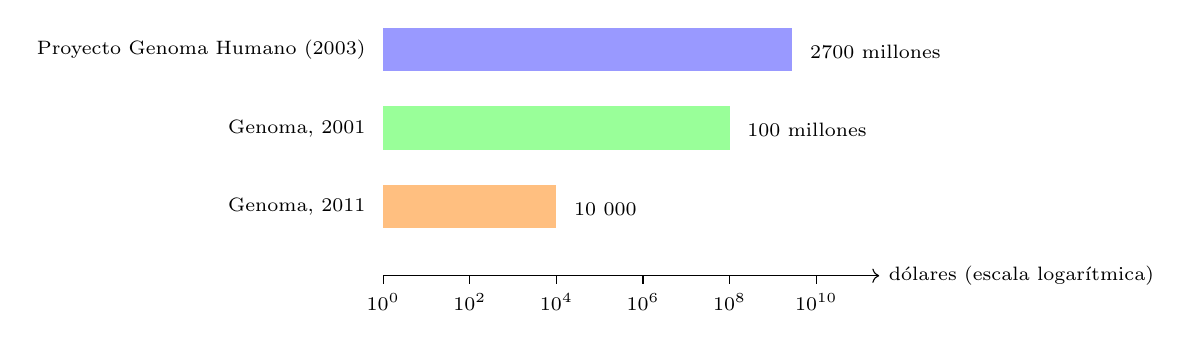
\begin{tikzpicture}

\def\bar#1#2#3#4{\fill[#4] (3.3,#1) rectangle ({3.3+#2*0.55},{#1+0.55}); \node[left, font=\scriptsize] at (3.2,{#1+0.27}) {#3}; }
\bar{3.0}{9.43}{Proyecto Genoma Humano (2003)}{blue!40}
\bar{2.0}{8}{Genoma, 2001}{green!40}
\bar{1.0}{4}{Genoma, 2011}{orange!50}
\foreach \e in {0,2,4,6,8,10} {\draw (3.3+\e*0.55,0.4) -- (3.3+\e*0.55,0.3) node[below, font=\scriptsize] {$10^{\e}$};}
\draw[->] (3.3,0.4) -- (9.6,0.4) node[right, font=\scriptsize] {dólares (escala logarítmica)};
\node[font=\scriptsize, right] at (8.6,3.25) {2700 millones}; \node[font=\scriptsize, right] at (7.8,2.25) {100 millones}; \node[font=\scriptsize, right] at (5.6,1.25) {10 000};

\end{tikzpicture}
\end{document}
